\documentclass[manuscript]{aastex}


\newcommand{\vdag}{(v)^\dagger}
\newcommand{\myemail}{eogorma@tcd.ie}


\shorttitle{The CO Shells of Betelgeuse}
\shortauthors{O'Gorman et al.}


\begin{document}


\title{CO in the Circumstellar Envelope of Betelgeuse with CARMA}

%% Use \author, \affil, and the \and command to format
%% author and affiliation information.
%% Note that \email has replaced the old \authoremail command
%% from AASTeX v4.0. You can use \email to mark an email address
%% anywhere in the paper, not just in the front matter.
%% As in the title, use \\ to force line breaks.

\author{Eamon O'Gorman and Graham M. Harper}
\affil{School of Physics, Trinity College Dublin, Dublin 2, Ireland}
\email{eogorma@tcd.ie}
\email{graham.harper@tcd.ie}
%\email{graham.harper@tcd.ie}


\author{Joanna M. Brown}
\affil{Harvard-Smithsonian Center for Astrophysics, 60 Garden Street, \\ MS-78, Cambridge, MA 02138, USA}
%\email{joannabrowne@cfa}

\and

\author{Alexander Brown}
\affil{Center for Astrophysics and Space Astronomy, University of Colorado, \\ 389 UCB, Boulder, CO 80309, USA}
%\email{alexander.brown@colorado.edu}

%% Mark off your abstract in the ``abstract'' environment. In the manuscript
%% style, abstract will output a Received/Accepted line after the
%% title and affiliation information. No date will appear since the author
%% does not have this information. The dates will be filled in by the
%% editorial office after submission.

\begin{abstract}
We report the first radio interferometric observations of the 1.3 mm emission line of $\rm{{}^{12}}$C$\rm{{}^{16}}O$ in the circumstellar envelope of the M supergiant $\alpha$ Ori.  Observations are made with the CARMA interferometer in the C, D, and E antenna configurations. We obtain excellent  uv-coverage (6 - 27 k$\lambda$) by combining data from all configurations allowing us to trace spatial scales from $0.8\arcsec$ to $4\arcsec$. The high spatial resolution C configuration map shows that the inner S1 shell has asymmetric outflow velocities of -10 km s${}^{-1}$ and +13 km s${}^{-1}$  with respect to the stellar rest frame. We find no evidence  for the outer S2 shell in this configuration and assume that this emission has been resolved out. The S2 shell appears as an extra blueshifted emission component in the D and E configuration maps between -10 km s${}^{-1}$  and -16 km s${}^{-1}$ but we see no trace of it in the redshifted velocity component. We conclude that the S2 shell is highly asymmetric in velocity space. A discrete off-source emission feature is detected at 5$\arcsec$ S-W of  $\alpha$ Ori in all D configuration maps. We image both shells in the combined map (all configurations) revealing their complex and irregular structure. We assign an outer radius of $\sim$5$\arcsec$ to S1 and believe that S2 may extend beyond our field of view of $\sim$12$\arcsec$. 
\end{abstract}

%% Keywords should appear after the \end{abstract} command. The uncommented
%% example has been keyed in ApJ style. See the instructions to authors
%% for the journal to which you are submitting your paper to determine
%% what keyword punctuation is appropriate.

\keywords{circumstellar matter --- Stars: individual: ($\rm{\alpha}$ Ori) --- Stars: late-type --- Stars: massive --- supergiants --- Radio lines: stars}

%% From the front matter, we move on to the body of the paper.
%% In the first two sections, notice the use of the natbib \citep
%% and \citet commands to identify citations.  The citations are
%% tied to the reference list via symbolic KEYs. The KEY corresponds
%% to the KEY in the \bibitem in the reference list below. We have
%% chosen the first three characters of the first author's name plus
%% the last two numeral of the year of publication as our KEY for
%% each reference.


%% Authors who wish to have the most important objects in their paper
%% linked in the electronic edition to a data center may do so by tagging
%% their objects with \objectname{} or \object{}.  Each macro takes the
%% object name as its required argument. The optional, square-bracket 
%% argument should be used in cases where the data center identification
%% differs from what is to be printed in the paper.  The text appearing 
%% in curly braces is what will appear in print in the published paper. 
%% If the object name is recognized by the data centers, it will be linked
%% in the electronic edition to the object data available at the data centers  
%%
%% Note that for sources with brackets in their names, e.g. [WEG2004] 14h-090,
%% the brackets must be escaped with backslashes when used in the first
%% square-bracket argument, for instance, \object[\[WEG2004\] 14h-090]{90}).
%%  Otherwise, LaTeX will issue an error. 

\section{Introduction}

Graham?

\section{Observations and Data Reduction}

The data were acquired with the 15 element CARMA (Combined Array for Research in Millimeter-wave Astronomy) interferometer which is located at Cedar Flat in eastern California and consists of nine 6.1 m antennas and six 10.4 m antennas. Table \ref{tab:tab1} summarizes our various tracks of millimeter observations which span the period 2007 May - 2009 November. The observations consist of on source profiles of the $\rm{{}^{12}}$C$\rm{{}^{16}}$O (J=2-1) line in the C, D and E array configurations. The baseline length spans over 30-350 m (C array), 11-150 m (D array) and 8-66 m (E array) providing spatial resolutions of 0.8$\arcsec$, 1.8$\arcsec$ and 4$\arcsec$ respectively at 1.3 mm. 

The receivers were tuned to the $\rm{{}^{12}}$C$\rm{{}^{16}}$O (J=2-1) line which has a rest frequency of 230.53 GHz (1.3 mm). The CARMA correlator takes measurements in three separate bands, each having an upper and lower sideband. One band was set to the low resolution 468 MHz   (with 15 channels) mode to observe continuum emission and was centered on the line. The other two bands were configured with 62 MHz and 31 MHz bandwidth across 63 channels (with a resolution of 1.3 km s$\rm{{}^{-1}}$ and 0.65 km s$\rm{{}^{-1}}$ respectively) and were also centered on the line. The line was measured in the upper sideband in the C and E array and in the lower sideband in the D array.

Bandpass and phase calibration were performed using 3C120 and 0530+135. 0532+075 was used as a secondary phase calibrator to determine the quality of the phase transfer from the primary phase calibrator. The observing sequence was to integrate on the primary phase calibrator for $\sim$ 2.5 minutes, the target for $\sim$ 18 minutes, and the secondary phase calibrator for $\sim$ 2.5 minutes. The cycle was repeated for each track which lasted between $\sim$ 1.5 hours and 5 hours. Absolute flux calibration was carried out using the bandpass and phase calibrators in the continuously updated CARMA flux catalog.

The raw data was initially Hanning smoothed within MIRIAD\footnote{Multichannel Image Reconstruction, Image Analysis and Display, \url{http://www.atnf.csiro.au/computing/software/miriad/}} and then exported into FITS format so that it could be analyzed with the CASA\footnote{Common Astronomy Software Applications, \url{http://casa.nrao.edu/}} data reduction package. All calibration and imaging was carried out within CASA. The image cubes  were multi-scale  CLEANed down to the 3.0$\rm{\sigma}$ threshold using natural weighting and were corrected for primary beam attenuation, unless otherwise stated below. The \textit{multiscale} algorithm \citep{rich08} within CASA was set to four unique scales; the largest corresponding to the the largest structures visible in individual channel maps. Each scale was approximately set to three times larger than the preceding scale. 
\section{Results} 

\subsection{Individual Configuration Image Cubes} \label{results1} % Link this label using \ref{results1}

The spectrum for each individual configuration image cube (which are composed of all the individual configuration tracks listed in Table \ref{tab:tab1}) can be used to obtain information on the kinematics of both shells. The three corresponding spectra are shown in Figure \ref{fig:fig1} for both the high (0.65 km s${}^{-1}$) and low (1.3 km s${}^{-1}$) resolution data and were obtained by extracting all emission within a circular area centered on the source. The radii for these circular areas were 1$\arcsec$, 4$\arcsec$ and 8$\arcsec$ for the C, D and E array image cubes respectively. The velocity rest frames of the spectra are plotted with respect to the stellar rest frame using a radial velocity of 20.7 km s${}^{-1}$  derived by \citet{harp08} .

The spectrum from the C array image cube has a total line width of $\sim$ 23 km s${}^{-1}$ and is dominated by three features; a blue wing, a red wing and a central emission feature at $\sim$ 0 km s${}^{-1}$. The blue wing of the CO emission profile extends to -10 km s${}^{-1}$ while the red wing extends to +13 km s${}^{-1}$. The spectra from the D and E array image cubes have an additional blue wing emission feature located between -10 km s${}^{-1}$ and -16 km s${}^{-1}$. This emission features appears to have been resolved out by the extended C antenna array which has a maximum scale of $\sim 4.5 \arcsec$. It is detected by the more compact configurations which are much more sensitive to extended emission. The total line width of the D and E array spectra are both $\sim$ 29 km s${}^{-1}$. In all three spectra the high and low resolution data match very well and this verifies the existence of the main emission features in these line profiles.

An additional spatially unresolved source is detected in the D configuration image cube and has been previously documented by \citet{harp09}. The component is present between $\sim$ -5 km s${}^{-1}$ and +6 km s${}^{-1}$ and is located $\sim$ 5$\arcsec$ S-W of $\alpha$ Ori. Its peak emission lies at $\sim$ 0 km s${}^{-1}$ and is approximately equal to 60$\%$ of the source peak emission. The corresponding channel maps in the E configuration image cube show extended emission out to ~8$\arcsec$ in the same S-W direction as shown in Figure \ref{fig:fig2}, but the source does not appear to be separate from $\alpha$ Ori. Curiously this second source does not appear in any of the C configuration image cube channel maps. 


\subsection{Multi-Configuration Image Cube} \label{results2} 

Figure \ref{fig:fig3} shows a subset of channel maps from the combined image cube. The first two channel maps show the continuum emission with no extended features apparent. Between -16 km s${}^{-1}$ and $\sim$-9 km s${}^{-1}$ we see evidence for the development of a classical shell. We first sample the highest velocity shell components where the emission is relatively compact (i.e. between $\sim$ -16 km s${}^{-1}$ and -13 km s${}^{-1}$) and then sample lower velocity components where the shell becomes a faint ring (i.e. between $\sim$ -12 km s${}^{-1}$ and -9 km s${}^{-1}$). These rings then either disappear into the noise of the channel maps or out of our field of view. Remarkable, this shell like structure is not seen in the corresponding red-shifted channel maps. All other channel maps out to a velocity of +13 km s${}^{-1}$ show some form of compact emission. This emission extends out to a maximum distance of $\sim$5$\arcsec$ but it is difficult to see evidence for shell development. 

The spectra in Figure \ref{fig:fig4} are taken from the combined image cube using circular extraction areas ranging in radius from 1$\arcsec$ to 10$\arcsec$. All spectra have a total linewidth of $\sim$29 km s${}^{-1}$ which is in close agreement with previous single dish observations (ref) of the line. The most striking feature of these spectra is the change in appearance of the blueshifted emission component located between -16 km s${}^{-1}$ and -10 km s${}^{-1}$.  At small extraction radii, where we sample the compact emission, this emission feature is weak in comparison to the rest of the line. However, as we take larger extraction radii, we begin to sample more and more of the extended emission and this emission feature gets stronger until it eventually becomes the dominant component of the line. 

\section{Discussion and Conclusions}

To do!

\acknowledgments

Support for CARMA construction was derived from the states of California, Illinois, and
Maryland, the James S. McDonnell Foundation, the Gordon and Betty Moore Foundation, the
Kenneth T. and Eileen L. Norris Foundation, the University of Chicago, the Associates of the
California Institute of Technology, and the National Science Foundation. Ongoing CARMA
development and operations are supported by the National Science Foundation under a
cooperative agreement, and by the CARMA partner universities.

%% After the acknowledgments section, use the following syntax and the
%% \facility{} macro to list the keywords of facilities used in the research
%% for the paper.  Each keyword will be checked against the master list during
%% copy editing.  Individual instruments or configurations can be provided 
%% in parentheses, after the keyword, but they will not be verified.

{\it Facilities:} \facility{CARMA}


%% The reference list follows the main body and any appendices.
%% Use LaTeX's thebibliography environment to mark up your reference list.
%% Note \begin{thebibliography} is followed by an empty set of
%% curly braces.  If you forget this, LaTeX will generate the error
%% "Perhaps a missing \item?".
%%
%% thebibliography produces citations in the text using \bibitem-\cite
%% cross-referencing. Each reference is preceded by a
%% \bibitem command that defines in curly braces the KEY that corresponds
%% to the KEY in the \cite commands (see the first section above).
%% Make sure that you provide a unique KEY for every \bibitem or else the
%% paper will not LaTeX. The square brackets should contain
%% the citation text that LaTeX will insert in
%% place of the \cite commands.

%% We have used macros to produce journal name abbreviations.
%% AASTeX provides a number of these for the more frequently-cited journals.
%% See the Author Guide for a list of them.

%% Note that the style of the \bibitem labels (in []) is slightly
%% different from previous examples.  The natbib system solves a host
%% of citation expression problems, but it is necessary to clearly
%% delimit the year from the author name used in the citation.
%% See the natbib documentation for more details and options.

\begin{thebibliography}{}
\bibitem[Harper et al.(2008)]{harp08} Harper, G. M., Brown, A., & Guinan, E. F. 2008, \aj, 135, 1430
\bibitem[Rich et al.(2008)]{rich08} Rich, J. W., de Blok, W. J. G., Cornwell, T. J. et al. 2008, \aj, 136, 2897
\bibitem[Harper et al.(2009)]{harp09} Harper, G. M., Carpenter, K. G., Ryde, N., et al. 2009, AIP Conf. Ser., 1094, 868

%\bibitem[Auri\`ere(1982)]{aur82} Auri\`ere, M.  1982, \aap,
%   109, 301
%\bibitem[Canizares et al.(1978)]{can78} Canizares, C. R.,
%   Grindlay, J. E., Hiltner, W. A., Liller, W., \&
%    McClintock, J. E.  1978, \apj, 224, 39
%\bibitem[Djorgovski \& King(1984)]{djo84} Djorgovski, S.,
%    \& King, I. R.  1984, \apjl, 277, L49
%\bibitem[Hagiwara \& Zeppenfeld(1986)]{hag86} Hagiwara, K., \&
%    Zeppenfeld, D.  1986, Nucl.Phys., 274, 1
\end{thebibliography}

\clearpage

\begin{figure}
%\centering
\epsscale{.80}
\plotone{fig1.eps}
\caption{Derived spectra from the image cubes of the final three different array configurations.\label{fig1}}
\label{fig:fig1}
\end{figure}

\clearpage
\begin{figure}
\mbox{
          \includegraphics[trim=0pt 10pt 40pt 10pt, clip, width=8.5cm]{apj.eps}
          \includegraphics[trim=0pt 10pt 40pt 10pt, clip, width=8.2cm]{apj_e.eps}
         }
\caption{(\textit{Left}) Integrated intensity image of the D configuration channel maps that contain the discrete second source. Contours for the integrated intensity are 1$\sigma$, 1.5$\sigma$, 3$\sigma$ and 4$\sigma$ (1$\sigma$ = 1.48 Jy beam${}^{-1}$ km s${}^{-1}$). (\textit{Right}) Integrated intensity image of the corresponding E configuration channel maps. Contours for the integrated intensity are again 1$\sigma$, 1.5$\sigma$, 3$\sigma$ and 4$\sigma$ (1$\sigma$ = 3.46 Jy beam${}^{-1}$ km s${}^{-1}$).}
\label{fig:fig3}
\end{figure}


\clearpage

\begin{figure}[hbt!]
%\centering
\mbox{
          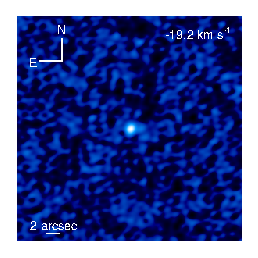
\includegraphics[]{f2.eps}
          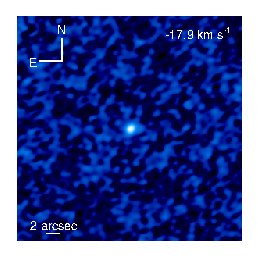
\includegraphics[]{f3.eps}
          }
\\
\mbox{
          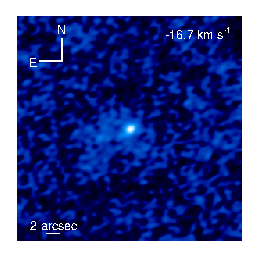
\includegraphics[]{f4.eps}
          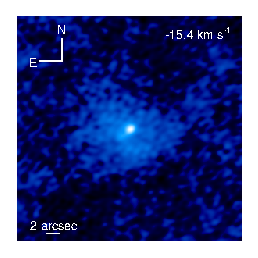
\includegraphics[]{f5.eps}
          }
\\
\mbox{
          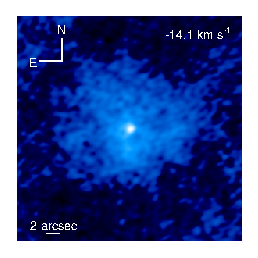
\includegraphics[]{f6.eps}
          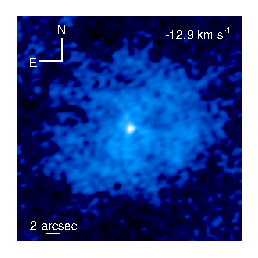
\includegraphics[]{f7.eps}
         }
\\
\mbox{
          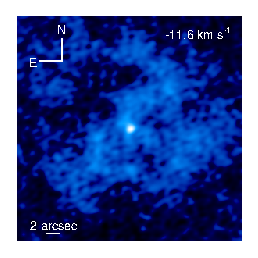
\includegraphics[]{f8.eps}
          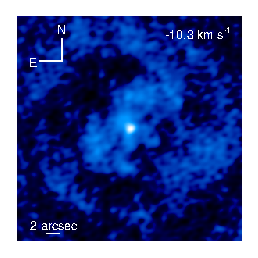
\includegraphics[]{f9.eps}
         }
\\
\mbox{
          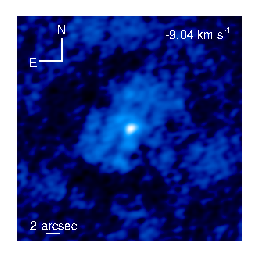
\includegraphics[]{f10.eps}
          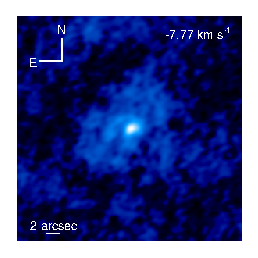
\includegraphics[]{f11.eps}
         }
\caption[]{10 channels from the final multi-configuration non-primary beam corrected image cube. The color scale has been normalized to the maximum and minimum value of each channel and is a function of the square root of the flux to emphasize the fainter emission.}
\label{fig:fig2}
\end{figure}


\clearpage

\begin{figure}
\epsscale{0.7}
\plotone{f13.eps}
\caption{Spectral profiles of the final combined image cube for circular extraction areas of radius 1$\arcsec$, 2$\arcsec$, 4$\arcsec$, 6$\arcsec$, 8$\arcsec$ and 10$\arcsec$.}
\label{fig:fig4}
\end{figure}

\clearpage

\begin{deluxetable}{ccccccc}
\tabletypesize{\scriptsize}
\tablecaption{CARMA Observations}
\tablewidth{0pt}
\tablehead{
\colhead{Observation} & \colhead{Configuration} & \colhead{Time on Source} & \colhead{Flux} 	& \colhead{Phase} & \colhead{Image Cube\tablenotemark{a}}\\
\colhead{Date}  	      & 		   	  & \colhead{(hr)} 		  & \colhead{Calibrator} & \colhead{Calibrators} & \colhead{Dynamic Range}}
}
\startdata
2007 May 11& D & 1.19 & 0530+135 & 0530+135, 0532+075 & 11.00 \\
2007 Jun 18 & D & 0.89 & 0530+135 & 0530+135, 0532+075 &  13.01 \\
2007 Jun 21 & D & 2.98 & 0530+135 & 0530+135, 0532+075 &  12.98 \\
2007 Jun 24 & D & 2.08 & 0530+135 & 0530+135, 0532+075 &  13.75 \\
2007 Jun 25 & D & 2.38 & 0530+135 & 0530+135, 0532+075 &  15.66 \\
2009 Jul 07 & E & 3.22 & 3C120 & 3C120, 0532+075 & 15.04 \\
2009 Nov 05 & C & 1.21 & 3C120 & 3C120, 0532+075 & 10.94 \\
2009 Nov 09 & C & 2.98 & 3C120 & 3C120, 0532+075 & 16.81 \\
2009 Nov 15 & C & 0.99 & 3C120 & 3C120, 0532+075 & 11.35 \\
2009 Nov 16 & C & 3.23 & 3C120 & 3C120, 0532+075 & 18.47  \\
All & C & 8.41 & \nodata & \nodata &   29.28 \\
All & D & 9.52 & \nodata & \nodata &   22.38 \\
All & All & 21.15 & \nodata & \nodata &   31.72 \\
\enddata
\tablenotetext{a}{Channel width of 1.3 km s$\rm{{}^{-1}}$ and not corrected for primary beam attenuation.}
\label{tab:tab1}
\end{deluxetable}


\end{document}

